\documentclass[a4paper,11pt]{article}
\usepackage[portuguese,algoruled,longend]{algorithm2e}
\usepackage{sobrapo-template}
\usepackage{amsmath,amssymb}
\usepackage{graphicx}
\usepackage[T1]{fontenc}
\usepackage{mathrsfs}
\usepackage{array}
\usepackage{rotating}
\usepackage{listings}


\usepackage[brazilian]{babel}
\usepackage[utf8]{inputenc}
\usepackage[T1]{fontenc}


\usepackage{indentfirst}

\title{\Large{Computação distribuída} \\ Relatório: Experimentação em ambiente nuvem}

\begin{document}

\maketitle


\author{
\name{Celio Henrique Nogueira Larcher Junior}
}

\vspace{1.0cm}

Serviços baseados em arquiteturas em nuvem vêm se tornando cada vez mais populares dado a praticidade e portabilidade que fornecem ao usuário. Este trabalho visa analisar a utilização para processamento intensivo de um entre os mais populares serviços o Amazon Web Services \cite{AWS}. 

Para isso, definiu-se uma aplicação baseada na resolução de sistemas lineares e através da configuração de clusters MPI, diversos experimentos foram realizados, verificando desempenho obtido por cada uma das combinações de VMs e comparando este fator ao custo das máquinas utilizadas. Desta forma foi possível obter um interessante comparativo entre as possibilidades de utilização do AWS como infraestrutura de experimentação.

\vspace{0.3cm}

\section{Aplicação utilizada}

\vspace{0.3cm}

Para experimentação foi utilizado o pacote NAS Parallel Benchmarks \cite{NAS}, um conjunto de aplicações desenvolvido pela NASA para avaliação de ambientes computacionais distribuídos. O NAS utiliza aplicações voltadas a simulação computacional da dinâmica de fluidos tendo, para cada uma das aplicações, variadas classes (dimensões de problemas) voltadas a atender as diferentes capacidades computacionais dos ambiantes testados.

No caso específico deste trabalho foi utilizada a aplicação denominada LU (Lower-Upper symmetric Gauss-Seidel) na versão classe C (relativa a computadores de tamanho padrão). 
A aplicação LU se utiliza de uma versão modificada do método de Gauss-Seidel para resolução de um sistema de diferenças finitas definido via versão discreta, instável e compressível das equações de Navier-Stokes em três dimensões espaciais. 
O método de Gauss-Seidel é um tradicional método iterativo para resolução de sistemas de equações lineares, dado pela forma:

$$x^{(k+1)}_i= \frac{1}{a_{ii}} \left( b_i - \sum_{j<i}a_{ij}x_j^{(k+1)} - \sum_{j>i}a_{ij}x_j^{(k)}\right), i=1,2,\dots,n$$

No caso desta implementação, são utilizadas as caraterísticas da matriz (como a simetria) de forma a reduzir o número de operações realizado. 

Para a classe C o tamanho da grid utilizada na definição do sistema de equações é de 102 x 102 x 102, tendo ainda um número de iterações de 250 para convergência do método. %e time step 2.0


\vspace{0.3cm}

\section{Processo de configuração do cluster}
\vspace{0.3cm}

Os experimentos foram realizados em ambientes clusters MPI definidos através do pacote MPICH \cite{MPI}. O MPI (\textit{Message Passing Interface}) é um padrão de comunicação de dados para programação paralela, voltado especialmente para aplicação em processamento distribuído. Possui várias implementações em diversas linguagens (C/C++, Java, Python, Fortran, $\dots$), sendo o MPICH uma opção \textit{open source} dentre as mais populares.


Para configuração do ambiente MPI foi feita a instalação do pacote em todas as máquinas virtuais participantes do cluster, o que, uma vez em posse do instalador do mesmo, é possível com apenas alguns comandos:

\begin{verbatim}
sudo apt-get install make gcc g++ gfortran  
./configure
make
sudo make install
echo "export LD_LIBRARY_PATH=/usr/local/lib" >> ~/.bashrc
sudo reboot
\end{verbatim}

Após a instalação, foi necessária a definição de uma chave RSA a ser compartilhada entre todas as máquinas do cluster de forma que as mesmas possam se comunicar livremente via MPI. Isto foi feito com a criação da chave em ambiente local e envio de uma cópia a todas as máquinas inseridas no cluster.

Ainda, em relação as configurações de acesso, no AWS foi necessário liberar as portas de comunicação entre as máquinas virtuais, o que foi feito através da inserção de todas em um mesmo \textit{Security Group} e a permissão de livre conexão entre as máquinas integrantes deste grupo (criação de uma nova regra de conexão liberando acesso a todas as portas entre as máquinas do grupo).


Uma outra opção explorada foi a configuração de um servidor NFS (\textit{Network File System}), o que permitiu manter uma unidade de disco compartilhada em rede entre diferentes máquinas. Desta forma as máquinas puderam compartilhar os mesmos executáveis a serem utilizados pelo MPI, sem necessidade de maiores cuidados em relação a organização dos arquivos em cada VM.


Por fim, com o serviço MPI devidamente configurado o \textit{benchmark} foi compilado em ambiente nuvem com o executável sendo compartilhado via interface NFS.

\vspace{0.3cm}

\section{Experimentos realizados}

\vspace{0.3cm}

Os experimentos foram realizados no ambiente AWS através de uma conta estudantil, o que, dado as limitações impostas a esta modalidade, não permitiu instanciar qualquer tipo de  máquina virtual, limitando as possibilidades de escolha. Neste sentido, a Tabela \ref{tab:inst} apresenta a configuração das instâncias utilizadas nos experimentos, bem como os preços individuais e o número de instâncias utilizadas em cada cluster. As instâncias de tipo t2 e m4 são voltadas a uso geral, tendo a instância m4 um melhor desempenho de rede quando comparada a t2, enquanto as instâncias t2 tem melhor desempenho computacional.




\begin{table}[htbp]
\center
\caption{Configuração das instâncias utilizadas e preço por instância}
\begin{tabular}{|l|r|r|r|r|}
\hline
 & \multicolumn{1}{c|}{\textbf{vCPU}} & \multicolumn{1}{c|}{\textbf{Memória (GiB)}} & \multicolumn{1}{c|}{\textbf{Preço (\$) / hora}} & \multicolumn{1}{l|}{\textbf{Instâncias / cluster}} \\ \hline
t2.micro & 1 & 1 & 0.0116 & 8 \\ \hline
t2.medium & 2 & 4 & 0.0464 & 4 \\ \hline
m4.large & 2 & 8 & 0.1 & 4 \\ \hline
m4.xlarge & 4 & 16 & 0.2 & 2 \\ \hline
t2.2xlarge & 8 & 32 & 0.3712 & 1 \\ \hline
\end{tabular}
\label{tab:inst}
\end{table}


Os clusters foram criados possuindo configuração homogênea (VMs com os mesmos tipos de instância) tendo como armazenamento um SSD com 8 GB. Foi definido ainda um alvo de 8 vCPUs por cluster de forma a tornar as comparações mais próximas. Desta forma, por exemplo, os experimentos executados na instância t2.2xlarge se utilizaram de apenas 1 VM, enquanto os experimentos executados na instância t2.micro foram compostos por 8 VMs.


O experimento consistiu de 5 execuções para cada configuração, de onde foi retirada a média dos tempos de execução. A Figura \ref{fig:tempoCluster} apresenta estes tempos para cada tipo de cluster.



\begin{figure}[h!]
	\center
	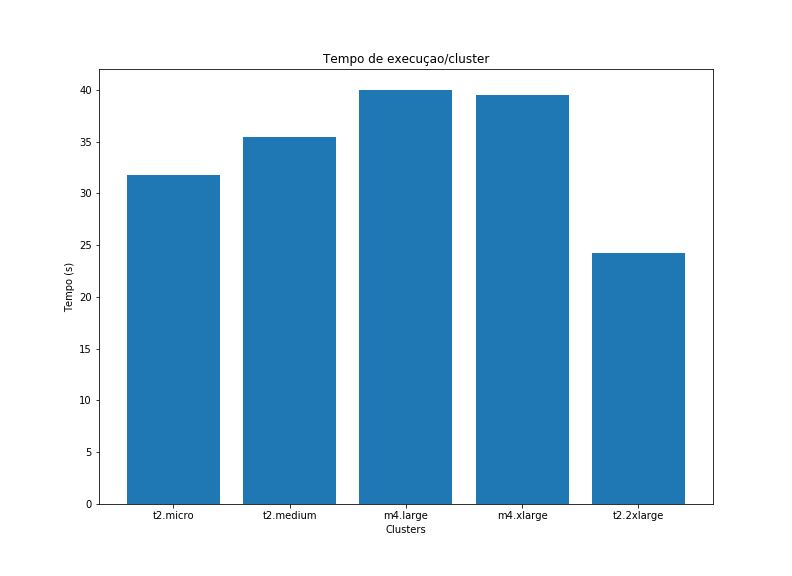
\includegraphics[scale=0.4]{figs/AllNodesTime.png}
	\caption{Média dos tempos de execução para cada tipo de cluster, considerando a utilização de 8 vCPUs}
	\label{fig:tempoCluster}
\end{figure}

Observando os resultados obtidos é interessante notar que para esta aplicação, não houve grande diferença de desempenho  entre os clusters analisados. De fato, a utilização de uma única instância do tipo t2.large possui o melhor desempenho, o que já era esperado dado ao menor \textit{overhead} de comunicação entre processos quando em uma mesma máquina. Nos demais resultados, a diferença mais expressiva está entre os \textit{clusters} do tipo t2 e do tipo m4, tendo as instâncias t2 um melhor resultado (o que é explicado pelas instâncias t2 possuírem melhor desempenho computacional). %quando comparado as instâncias m4. 
%Da mesma forma, as instâncias t2, por possuírem a possibilidade de realizar busts Mas o mesmo não é observado para as demais configurações, com a utilização de 8 instâncias do tipo t2.micro apresentando o segundo melhor desempenho.

Ainda, é importante comentar que para as instâncias t2.micro e t2.medium foi observado uma maior variação de desempenho, tendo algumas execuções (não incluídas no relatório) com tempo completamente divergente da média de execução. Isso provavelmente se deve a não haver uma garantia de recursos neste tipo de instância, não sendo capaz de atingir em todos os momentos seu pico de desempenho.%, podendo ocorrer momentos de grande disputa de recurso no cluster da AWS, além da possibilidade de congestionamento na rede interna.

Utilizando os mesmos dados deste experimento, a Figura \ref{fig:precoCluster} trás uma estimativa do preço pago pelo tempo de computação realizado. No caso, foi utilizado o preço por instância multiplicado pelo número de instâncias do cluster e ponderado pelo tempo de execução.


\begin{figure}[h!]
	\center
	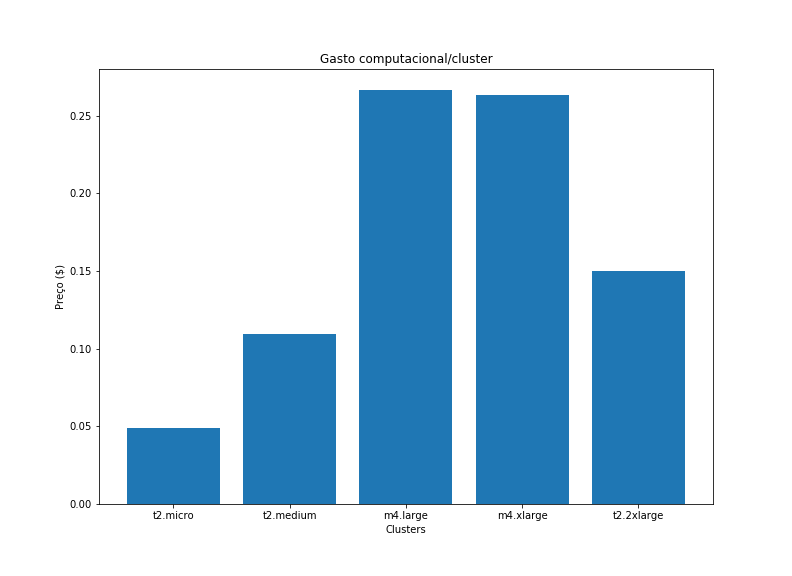
\includegraphics[scale=0.4]{figs/AllNodesPreco.png}
	\caption{Preço médio de execução para cada tipo de cluster, considerando a utilização de 8 vCPUs}
	\label{fig:precoCluster}
\end{figure}

\vspace{0.4cm}

Neste segundo comparativo, as instâncias do tipo t2 se destacam (especialmente t2.micro) dado estas possuírem um custo menor de utilização (tendo por outro lado um pior desempenho de rede). No caso desta aplicação, a melhor performance de rede aparentemente não gerou um benefício suficiente para que valha o custo maior das instâncias (o que provavelmente não é verdadeiro para outras aplicações que demandem um maior volume de transferência de dados). Verificando este fator, a utilização de uma configuração distribuída ainda apresentou um custo menor quando comparada a uma única instância (t2.xlarge), mas tendo que se considerar que no \textit{benchmark} as execuções não levam em conta possíveis otimizações para a configuração multicore (utilização de OpenMP e Pthreads x MPI).

Por fim, a Tabela \ref{fig:tempot2micro} apresenta o desempenho com diferentes números de instâncias inseridas no cluster MPI, considerando instâncias t2.micro.


\begin{figure}[h!]
	\center
	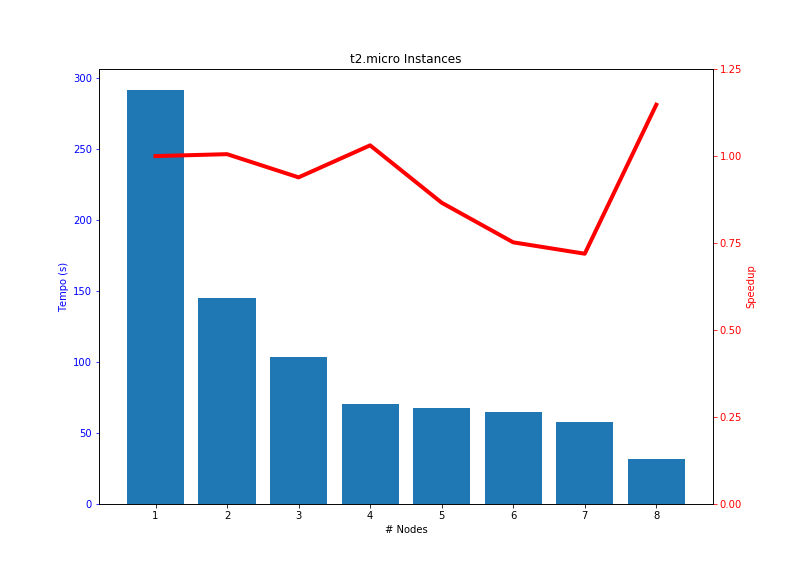
\includegraphics[scale=0.4]{figs/t2microTime.png}
	\caption{Média dos tempos de execução (colunas em azul) e speedup (linha em vermelho)  para diferentes números de instâncias com configuração t2.micro}
	\label{fig:tempot2micro}
\end{figure}

Observando os tempos de execução, é possível reparar um grande ganho de desempenho com o incremento do número de instâncias (especialmente nas configurações com 2, 4 e 8 instâncias, o que provavelmente indica uma melhor divisão de tarefas nestes patamares). 
Neste sentido, a paralelização do código em MPI apresenta bom desempenho, com utilização de um número maior de VMs. Ainda, é estranho a princípio notar pontos de speedup com valor maior que 1 (limite teórico), mas isto provavelmente se deve a limitações da instância (apenas 1GB de RAM), o que faz com que haja um melhor desempenho simplesmente pelos dados estarem distribuídos e totalmente inseridos em memória.

\vspace{0.3cm}

\section{Comentários acerca dos experimentos}

\vspace{0.3cm}


O experimento realizado não busca, de nenhuma forma, apresentar uma conclusão definitiva acerca da melhor configuração a ser utilizada, sendo a escolha muito dependente da demanda apresentada por cada aplicação. Apesar disso, foi interessante notar que a utilização de um cluster MPI composto por máquinas de menor desempenho pode ser uma opção a ser considerada (especialmente se orçamento for um fator importante). 
Na aplicação em questão pode-se observar que dado a boa capacidade de paralelização do código, a opção de um cluster MPI é factível, não havendo uma perda de desempenho grande gerada pela comunicação.


Por outro lado, no caso geral a utilização de uma instância de  maior capacidade computacional será  provavelmente a escolha mais adequada, dado o menor tempo de computação, uma maior garantia de desempenho (sofrendo menor interferência  de outros fatores como a capacidade da rede local) e por não haver uma diferença absurda no valor pago por esse poder computacional a mais (especialmente considerando as otimizações possibilitadas por esta opção). 

Ainda, é importante citar que as instâncias otimizadas para computação (tipos c4 e c5) podem apresentar uma melhor relação de custo benefício quando comparadas as de uso geral (t2 e m4), o que não foi possível observar nestes experimentos. Apesar disso, pode ser razoável considerar que ao menos para a escolha entre a criação de um cluster MPI ou utilização de uma única instância de poder computacional equivalente, possa haver um paralelo ao observado neste experimento sendo a criação de um cluster MPI uma opção viável para algumas situações.



\vspace{0.5cm}

\begin{thebibliography}{99}

\vspace{0.5cm}

%	 \bibitem{Zucchini00}
%	Zucchini W. (2000). 
%	\newblock{ An Introduction to Model Selection. \em Journal of Mathematical Psychology}



	 \bibitem{AWS}
	Amazon AWS Educate
	\newblock{\em https://www.awseducate.com/student/s/}

	 \bibitem{MPI}
	MPICH 
	\newblock{\em https://www.mpich.org/}


	 \bibitem{NAS}
	NAS Parallel Benchmarks
	\newblock{\em https://www.nas.nasa.gov/publications/npb.html}








\end{thebibliography}




\end{document}

